% ser-2017-aha-slcs.Rnw

%---------------------------------------------------------------
% Preamble
% --------------------------------------------------------------
%
% NOTE: See rice-sample.tex written by Daina Chiba at Rice University for formatting and preamble code that I copied, http://ricebeamer.dynaman.net/
\documentclass[final]{beamer}\usepackage[]{graphicx}\usepackage[]{color}
%% maxwidth is the original width if it is less than linewidth
%% otherwise use linewidth (to make sure the graphics do not exceed the margin)
\makeatletter
\def\maxwidth{ %
  \ifdim\Gin@nat@width>\linewidth
    \linewidth
  \else
    \Gin@nat@width
  \fi
}
\makeatother

\definecolor{fgcolor}{rgb}{0.345, 0.345, 0.345}
\newcommand{\hlnum}[1]{\textcolor[rgb]{0.686,0.059,0.569}{#1}}%
\newcommand{\hlstr}[1]{\textcolor[rgb]{0.192,0.494,0.8}{#1}}%
\newcommand{\hlcom}[1]{\textcolor[rgb]{0.678,0.584,0.686}{\textit{#1}}}%
\newcommand{\hlopt}[1]{\textcolor[rgb]{0,0,0}{#1}}%
\newcommand{\hlstd}[1]{\textcolor[rgb]{0.345,0.345,0.345}{#1}}%
\newcommand{\hlkwa}[1]{\textcolor[rgb]{0.161,0.373,0.58}{\textbf{#1}}}%
\newcommand{\hlkwb}[1]{\textcolor[rgb]{0.69,0.353,0.396}{#1}}%
\newcommand{\hlkwc}[1]{\textcolor[rgb]{0.333,0.667,0.333}{#1}}%
\newcommand{\hlkwd}[1]{\textcolor[rgb]{0.737,0.353,0.396}{\textbf{#1}}}%
\let\hlipl\hlkwb

\usepackage{framed}
\makeatletter
\newenvironment{kframe}{%
 \def\at@end@of@kframe{}%
 \ifinner\ifhmode%
  \def\at@end@of@kframe{\end{minipage}}%
  \begin{minipage}{\columnwidth}%
 \fi\fi%
 \def\FrameCommand##1{\hskip\@totalleftmargin \hskip-\fboxsep
 \colorbox{shadecolor}{##1}\hskip-\fboxsep
     % There is no \\@totalrightmargin, so:
     \hskip-\linewidth \hskip-\@totalleftmargin \hskip\columnwidth}%
 \MakeFramed {\advance\hsize-\width
   \@totalleftmargin\z@ \linewidth\hsize
   \@setminipage}}%
 {\par\unskip\endMakeFramed%
 \at@end@of@kframe}
\makeatother

\definecolor{shadecolor}{rgb}{.97, .97, .97}
\definecolor{messagecolor}{rgb}{0, 0, 0}
\definecolor{warningcolor}{rgb}{1, 0, 1}
\definecolor{errorcolor}{rgb}{1, 0, 0}
\newenvironment{knitrout}{}{} % an empty environment to be redefined in TeX

\usepackage{alltt}
\usepackage[orientation=landscape, size=custom, width=121.92, height=106.68, scale=1.7]{beamerposter}  % this matches 4 feet (48 inches) by 3.5 feet (42 inches). Will get from phdposters.com 1 inch per 2.54 cm

\mode<presentation>{\usetheme{UNC5}}
\usepackage[english]{babel}
\usepackage[latin1]{inputenc}
\usepackage{bm}
\usepackage{blindtext}
\usepackage{scrextend}
\addtokomafont{labelinglabel}{\sffamily}
\usepackage{csquotes}
\usepackage{booktabs}

\setbeamercolor{bibliography entry title}{fg=black,bg=black}% see http://tex.stackexchange.com/questions/71352/beamer-undefined-color-local-structure
\setbeamertemplate{caption}[numbered]

% got from http://tex.stackexchange.com/questions/48023/mimic-bibtex-apalike-with-biblatex-biblatex-apa-broken
\PassOptionsToPackage{
        style=numeric,
        hyperref=true,
        backend=bibtex,
        maxbibnames=1,
        firstinits=true,
        uniquename=init,
        maxcitenames=2,
        parentracker=true,
        url=false,
        doi=true,
        isbn=false,
        eprint=false,
        backref=false,
            }{biblatex}
% see the following link for info on biblatex sort order issue: 
% http://tex.stackexchange.com/questions/51434/biblatex-citation-order
\usepackage[natbib=true, sorting=none, style=numeric, backend=biber]{biblatex}
\addbibresource{lit}
\renewcommand*{\bibfont}{\scriptsize}

%\usepackage{fontspec} % have to compile with XeLaTeX
%\setmainfont{Arial}
\usepackage[T1]{fontenc}
\usepackage{helvet}
\renewcommand{\familydefault}{\sfdefault} % get something like Arial

\usepackage{amsmath,amsthm, amssymb, latexsym}
\usepackage{wrapfig}

\usepackage{array,booktabs,tabularx}
\newcolumntype{Z}{>{\centering\arraybackslash}X} % centered tabularx columns

\usepackage[shortlabels]{enumitem}

% \setlist[description]{style=nextline}
\setlist[itemize]{leftmargin=0.55in, labelindent=16pt, label=$\bullet$}

\usepackage[framemethod=TikZ]{mdframed}
\mdfdefinestyle{MyFrame}{%
    linecolor=carolinablue,
    outerlinewidth=4pt,
    roundcorner=20pt,
    innerrightmargin=20pt,
    innerleftmargin=20pt,
    backgroundcolor=carolinablue!20}
    
% comment 
\newcommand{\comment}[1]{}

% (relative) path to the figures
\graphicspath{{figs/}}

\newlength{\columnheight}
\setlength{\columnheight}{105cm}
\newlength{\sepwid}
\newlength{\onecolwid}
\newlength{\twocolwid}
\newlength{\threecolwid}
\setlength{\sepwid}{0.024\paperwidth}
\setlength{\onecolwid}{0.31\paperwidth}
\setlength{\twocolwid}{0.31\paperwidth}
\setlength{\threecolwid}{0.31\paperwidth}





% This is based on the template at http://www-i6.informatik.rwth-aachen.de/~dreuw/latexbeamerposter.php

% --------------------------------------------------------------------------------------% 
% Title, author, date, etc.
% --------------------------------------------------------------------------------------% 
% see http://tex.stackexchange.com/questions/9740/how-can-i-add-vertical-space-to-a-beamercolorbox-to-make-it-align-with-another-o
\title{Lipid-related Genetic Variants and Lipid Outcomes in a Cohort of Chilean Children} 
\author[vonholle@unc.edu]{Ann Von Holle, Anne Justice, Misa Graff, Kari North, UNC, Chapel Hill, NC; Estela Blanco, Sheila Gahagan, UCSD, San Diego, CA; B\'arbara Angel, Unidad de Nutrici\'on P\'ublica INTA, Univ de Chile, Santiago, Chile; Jos\'e Luis Santos, Pontificia Univ Cat\'olica de Chile, Santiago, Chile}
\institute{UNC}
\titlegraphic{unc-black.eps} %this is the path to your logo

% -------------------------------------------------------------------------------------%
% Contents
% -------------------------------------------------------------------------------------%
\IfFileExists{upquote.sty}{\usepackage{upquote}}{}
\begin{document}
\setlength{\parfillskip}{0pt plus 1fil}


\begin{frame}[t]

  \begin{columns}[T] % t instead of T or c means columns start at top

    % ---------------------------------------------------------%
    % Set up 1st column
    % ---------------------------------------------------------%
    \begin{column}{\onecolwid}
    \begin{beamercolorbox}[wd=\textwidth]{postercolumn}
    % fill each column with content
        % -----------------------------------------------------------
        % 1-1 (first column's first block
        % -----------------------------------------------------------
        % fill each column with content
        \begin{block}{Introduction}

          Lipid concentrations:
        
          \begin{itemize}
                \begin{itemize} \normalsize
                    \item Are a recognized heritable risk factor for cardiovascular disease (CVD)
                    \item Associate with >150 loci in adults
                    \item Vary across ancestral groups
                    \item Include high density lipoprotein cholesterol (HDL-C), low density lipoprotein cholesterol (LDL-C) and triglycerides (TG).
                    \end{itemize}
            \item Genetic architecture underlying lipid traits is similar across ancestral groups for adults.
            \item Sparse research in younger age groups motivates further investigation.
            \end{itemize}
    
        \end{block}
        \vskip1ex
    
        % -----------------------------------------------------------
        % 1-2
        % -----------------------------------------------------------
        \begin{block}{Aims}
        
        \setbeamertemplate{itemize items}[square]
        
          \begin{enumerate}[1.]
            \item To estimate association between:
            \begin{itemize}
                \item Lipid risk variants first identified in adults and adolescent traits.
                \item Lipid traits of adolescents from a Chilean infancy cohort.
              \end{itemize}
            \item Compare results across Chilean and Finnish cohorts.
            \end{enumerate}

        \end{block}
        \vskip1ex

        % -----------------------------------------------------------
        % 1-3
        % -----------------------------------------------------------

        
        \begin{block}{Sample}
        
\vspace{-1em}
        
% see http://tex.stackexchange.com/questions/208429/problem-with-wrapfig-and-itemize
\begin{itemize}
    \parbox[t]{\dimexpr\textwidth-\leftmargin}{%
\raggedright
      \begin{wrapfigure}[10]{r}{0.5\textwidth}
        \centering
        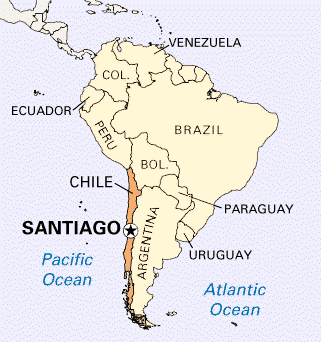
\includegraphics[width=\linewidth]{santiago-map.png}
      \end{wrapfigure}
          \item Santiago Longitudinal Cohort Study (n=1645), 1991-1996
          \item \raggedright Current sample recruited from n=888, which were 2/3 RCT groups
          \item  n=677 with infancy and adolescent data (average age = 17 years) and of those n=546 with genotyped data in analyses that follow
          \item  Low to middle income
          \item Ethnically mixed American Indian and Spanish descent families
          \item Lipid traits measured after overnight fasting
    }
  \end{itemize}

 
        
        \end{block}

  \end{beamercolorbox}
  \end{column}
    % ---------------------------------------------------------%
    % end the 1st column
    % ---------------------------------------------------------%

% ---------------------------------------------------------%
% Set up 2nd column
% ---------------------------------------------------------%

\begin{column}{\twocolwid}
\begin{beamercolorbox}[center,wd=\textwidth]{postercolumn}

        % -----------------------------------------------------------
        % 2-1
        % -----------------------------------------------------------
        \begin{block}{Methods}
        
        \begin{enumerate}[1.]
          \item Test additive association between lipid traits and adequately powered single risk variants.
            \begin{itemize}
              \item 76 common \textbf{lipid variants} selected from a European genome-wide meta-analysis with strongest independent signal.
              \item Association tests include \textbf{single variants} with \textit{a priori} power > 0.80.
            \end{itemize}
          \item Assess the association of weighted polygenic risk scores (wPRS) on lipid traits using additive linear regression model.
              \begin{itemize}
                      \item \textbf{Coefficients} for wPRS and power calculations based on European adult association studies (4).
              \end{itemize}

          \item Characterize proportion of variance explained by lipid variants.
          \end{enumerate}
% \vskip0.5em
% \toprule[2mm]
% \vskip0.5em

        \end{block}
        \vskip1ex

        % -----------------------------------------------------------
        % 2-2
        % -----------------------------------------------------------
        \begin{block}{Results}
        
        % First figure
        % %%%%%%%%%%%%%%%%%%%%%%%%%%%%%%%%%%%%%%%%%%%%%%%%%%


        % Point to code to make all tables from summary statistics run on Kure
        % These figures were originally made for Dec 2016 presentation
        



        % Run code chunk from tables-slides.R to make table from summary statistics run on Kure


        


\vskip-0.2em

# Figure 1. Candidate single variant tests of association by variant and sample
% NOTE: these were determined via power calculations at ~\Documents\dissertation\unc-dissertation-markdown\includes\scripts\power-calcs-ind-assoc.Rmd
        \centering
        \begin{figure}
%        \caption{Candidate single variant tests of association by variant and sample}


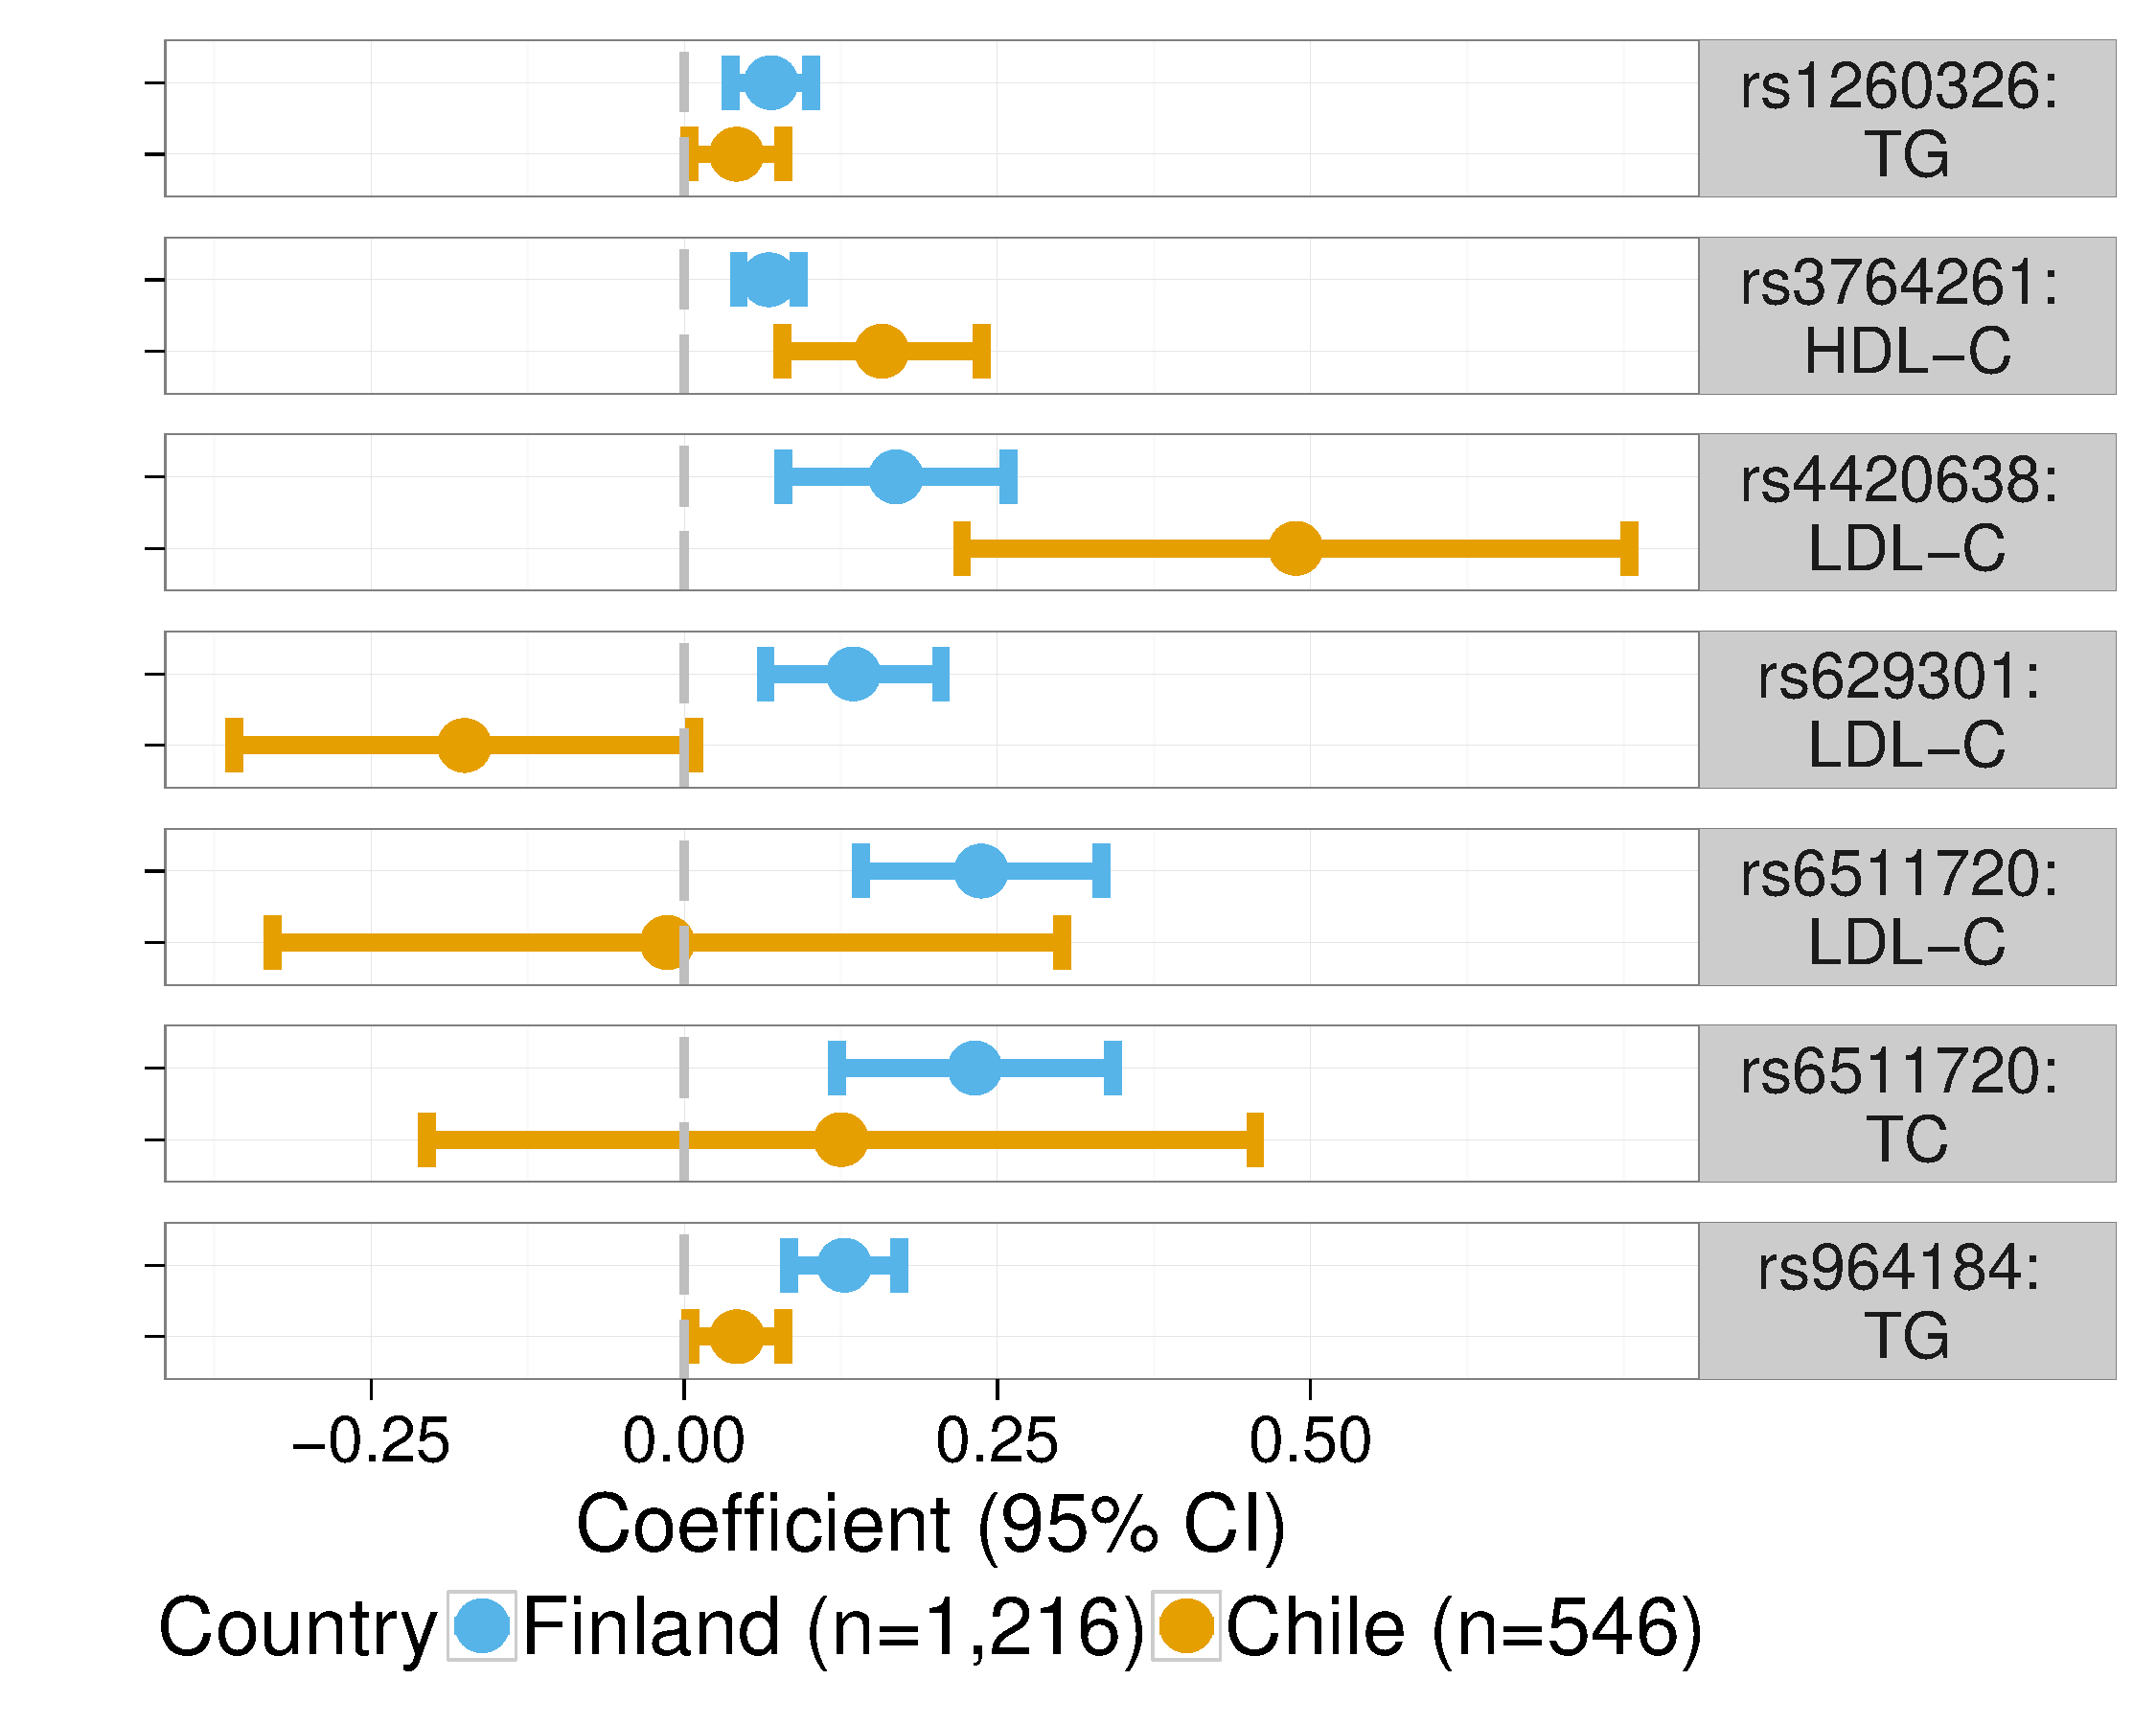
\includegraphics[width=\maxwidth]{figure/fig-assoc-2-poster-1} 

        \end{figure}
        
            \begin{itemize}
            \item \raggedright  Majority of single variants tested in Chilean sample have concordant direction of associations.
              \begin{itemize}
                \item Two LDL-C variants in opposite direction.
                \end{itemize}
              \end{itemize}



        \end{block}

\end{beamercolorbox}
\end{column}

% ---------------------------------------------------------%
% end the 2nd column


% ---------------------------------------------------------%
% Set up 3rd column
% ---------------------------------------------------------%

\begin{column}{\threecolwid}
\begin{beamercolorbox}[center,wd=\textwidth]{postercolumn}


        \vfill

        % -----------------------------------------------------------
        % 3-1
        % -----------------------------------------------------------
        \begin{block}{Results, cont...}
        
        
          
        % Second figure
        % %%%%%%%%%%%%%%%%%%%%%%%%%%%%%%%%%%%%%%%%%%%%%%%%%%
        \centering
# Figure 2. wPRS regression coefficients by sample and sex

% Run code chunk from tables-slides.R to make table from summary statistics run on Kure



        \begin{figure}
\begin{knitrout}
\definecolor{shadecolor}{rgb}{0.969, 0.969, 0.969}\color{fgcolor}
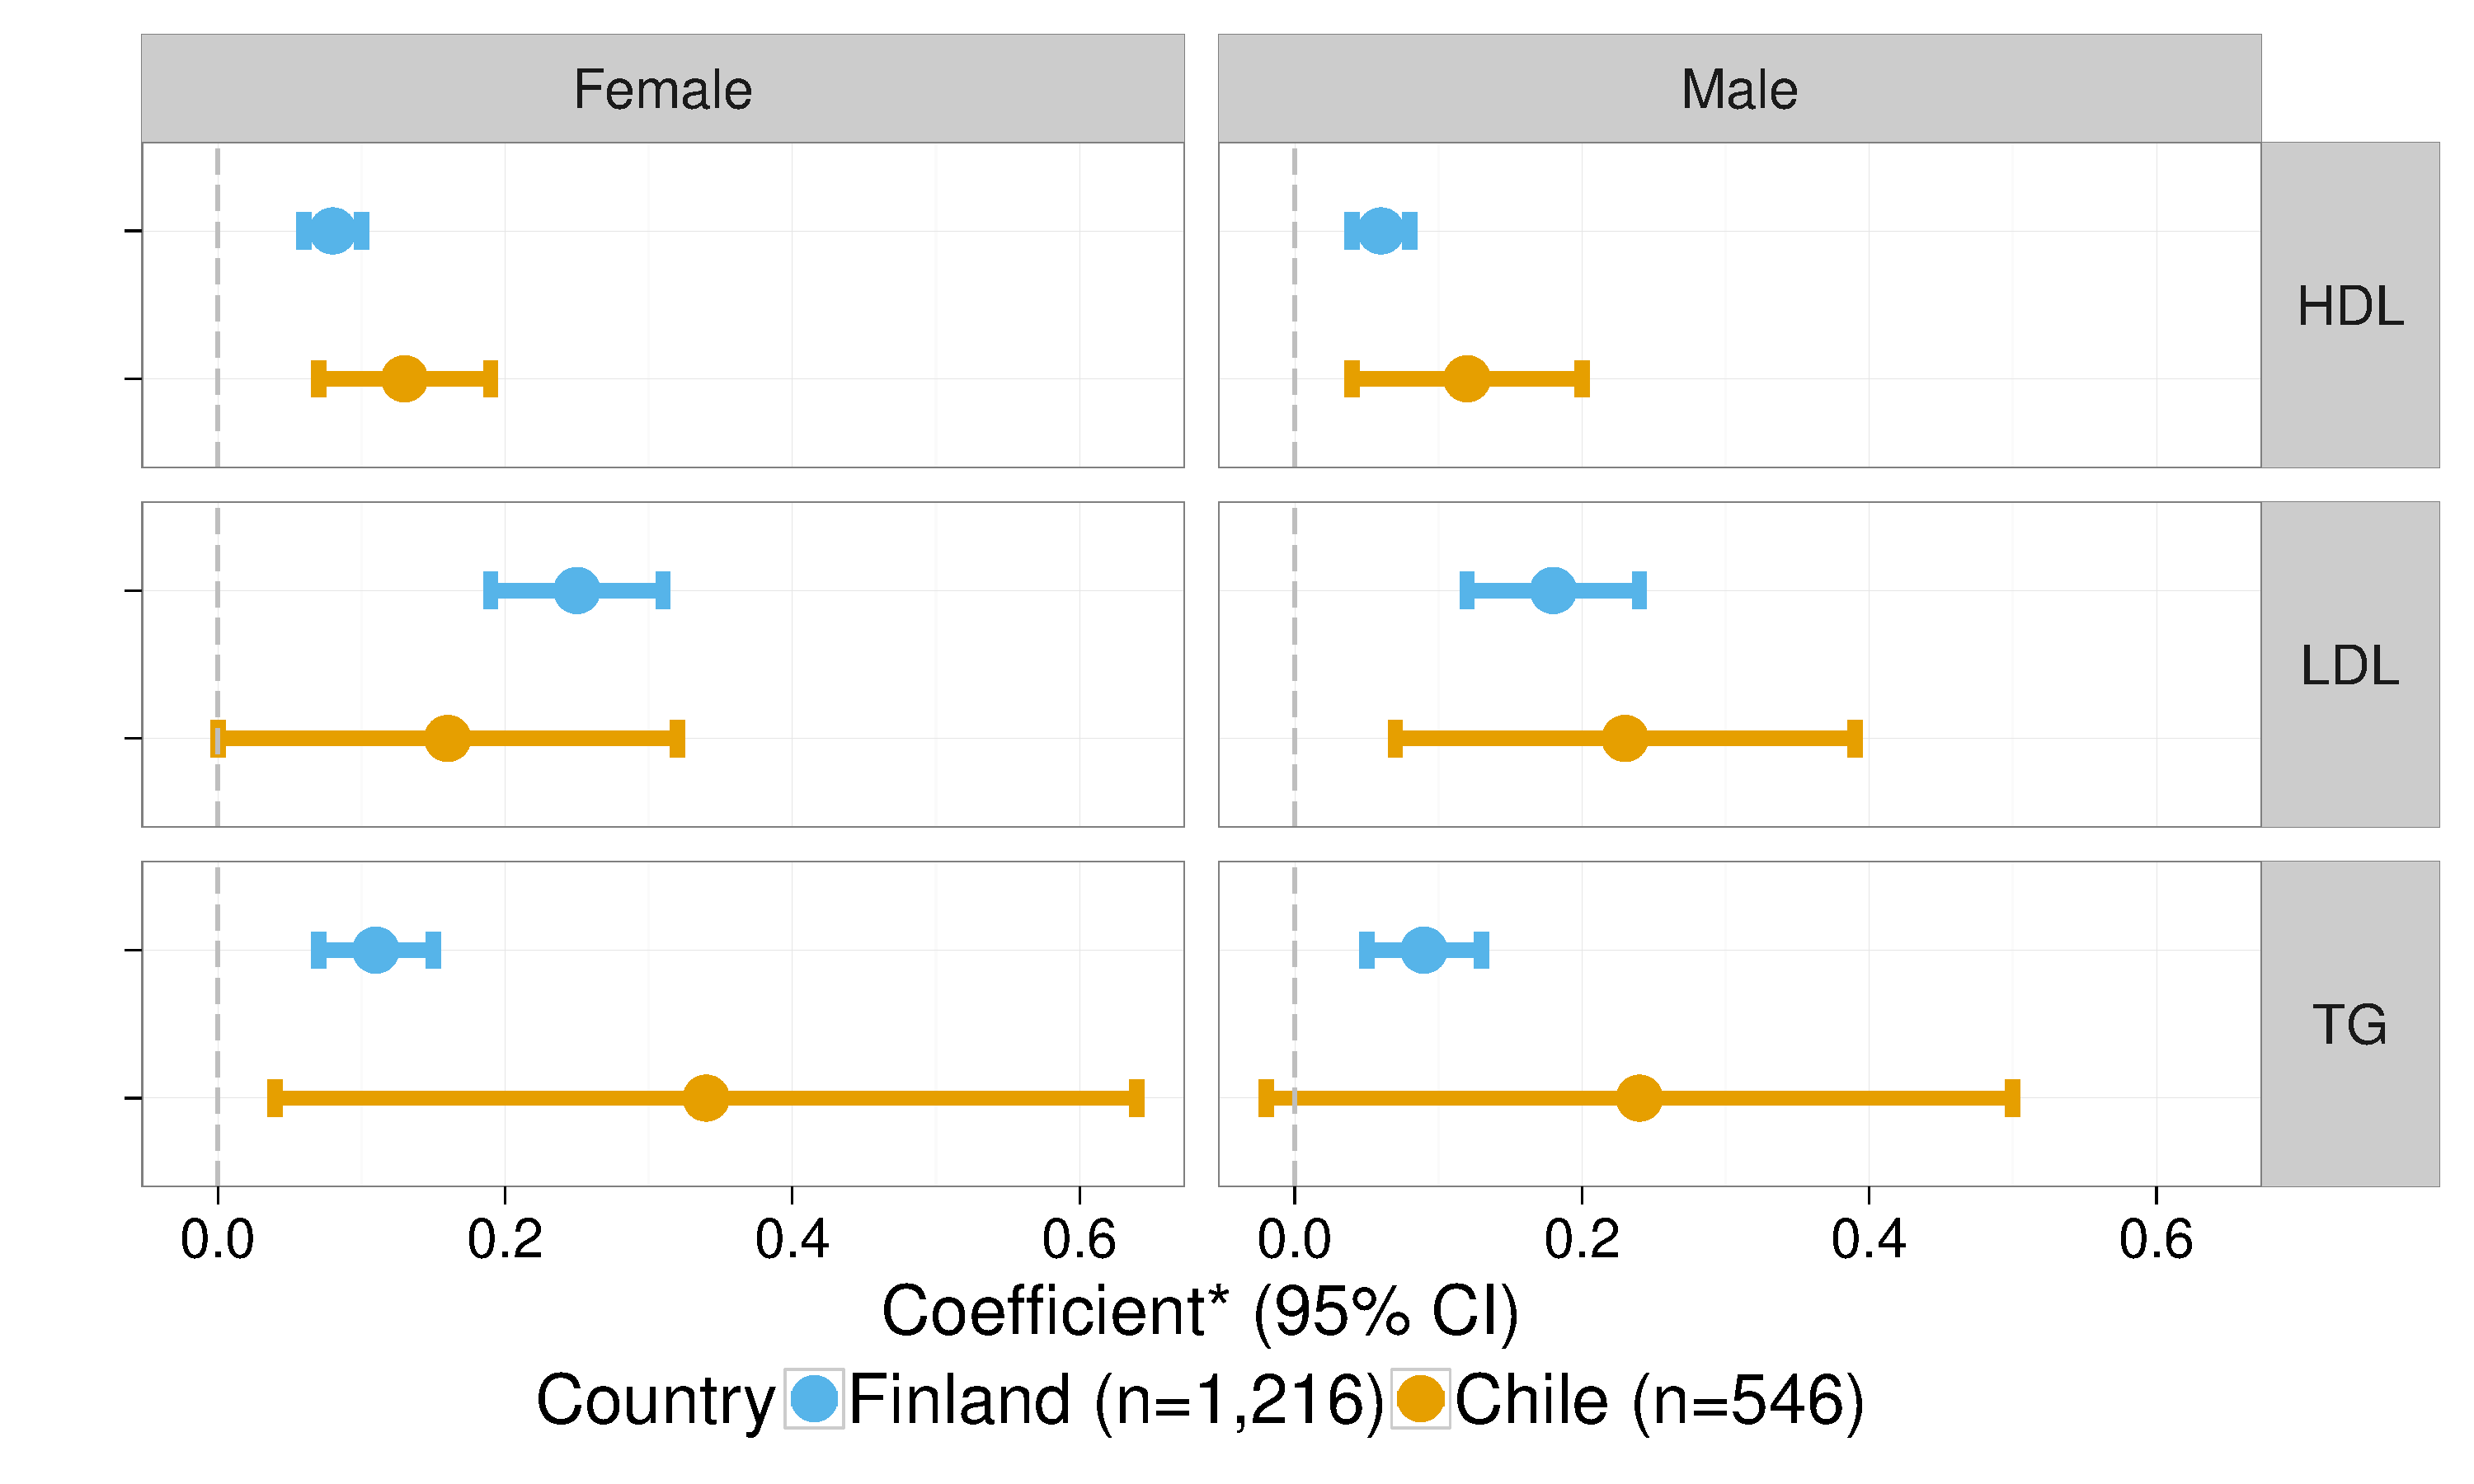
\includegraphics[width=\maxwidth]{figure/fig3-2-poster-1} 

\end{knitrout}
        \end{figure}
        
        
\vspace{-0.4em}
        
        \begin{addmargin}[2cm]{0cm}
        \begin{flusChileaneft}
        \footnotesize{*Coefficients represent change in outcome per 1 SD change in wPRS, adjusted for first five principal components representing ancestry but NOT BMI.}
        \end{flusChileaneft}
        \end{addmargin}
        
        \begin{itemize}
            \item \raggedright  wPRS has stronger association for each lipid outcome in Chilean versus Finnish sample except LDL-C for females.
            \end{itemize}
\vskip0.5em

        % Third figure
        % %%%%%%%%%%%%%%%%%%%%%%%%%%%%%%%%%%%%%%%%%%%%%%%%%%

% Run code chunk from tables-slides.R to make table from summary statistics run on Kure


        

        # Figure 3. Proportion of lipid traits variance explained by lipid-related variants, by sex
        \centering
        \begin{figure}

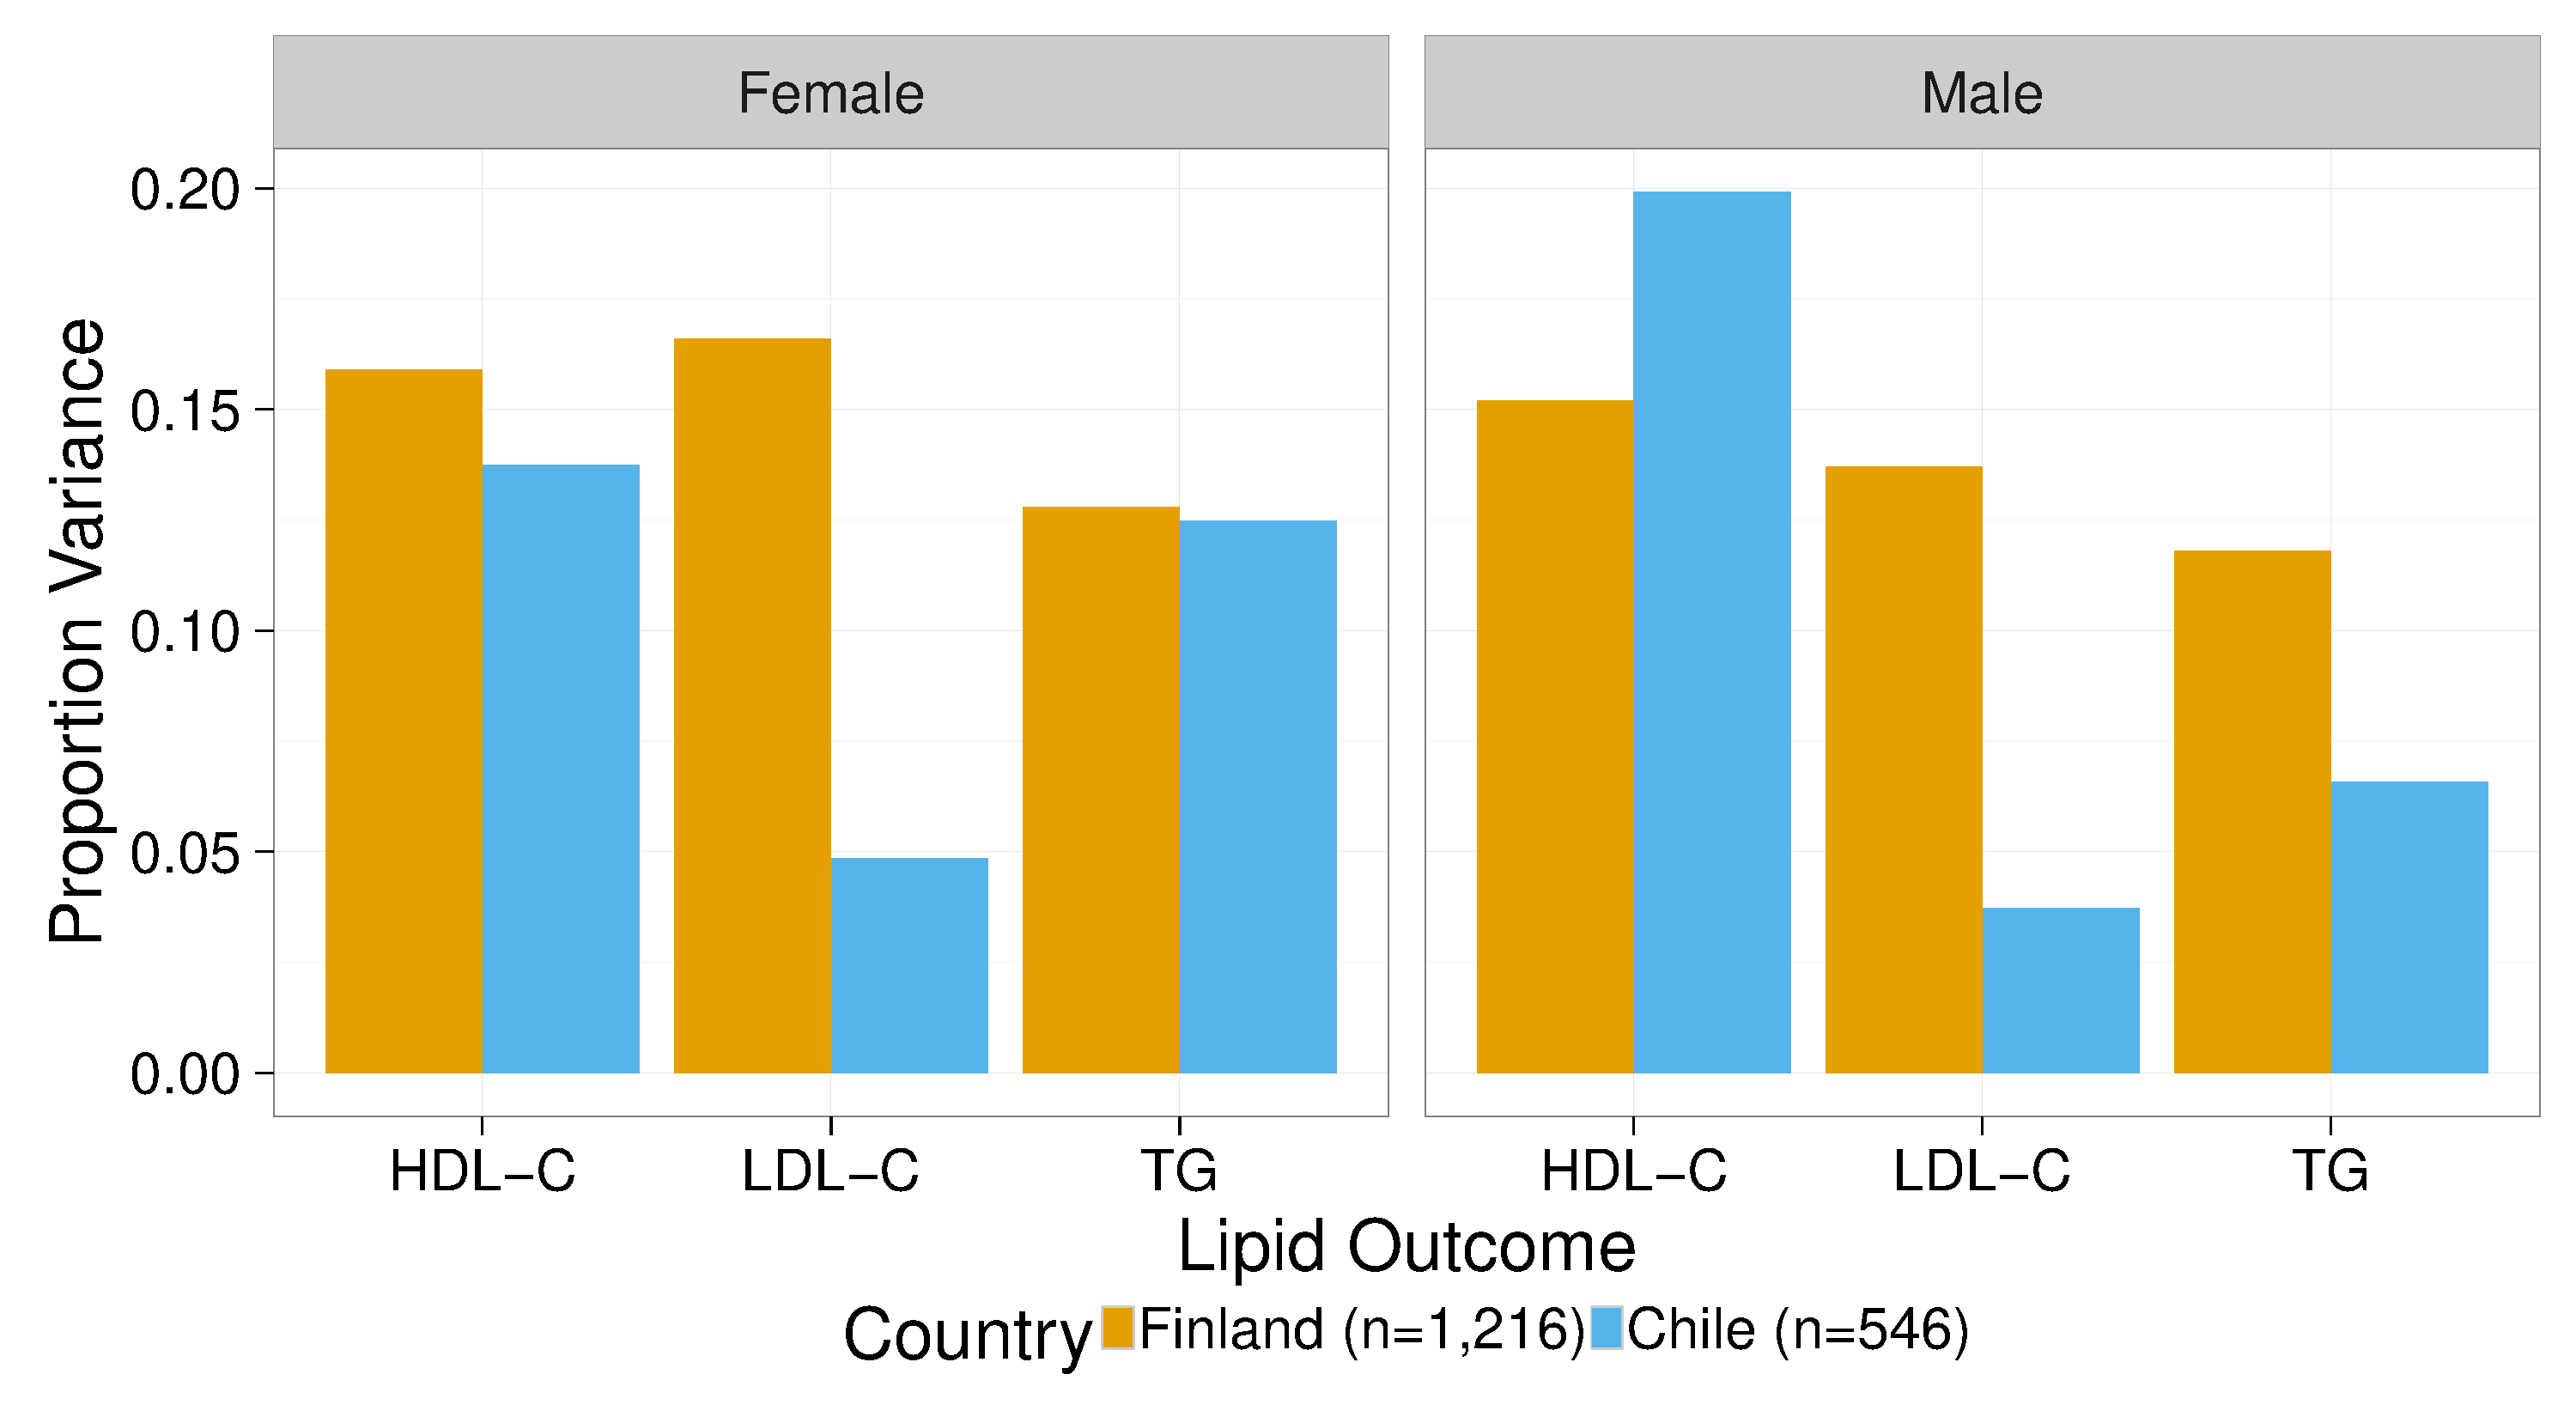
\includegraphics[width=\maxwidth]{figure/fig2-2poster-1} 

        \end{figure}

%        \begin{mdframed}[style=MyFrame]
          \begin{itemize}
            \item \raggedright LDL-C-related variants explain much less variance in Chilean sample.
            \end{itemize}
%            \end{mdframed}
        
        \end{block}
        
        \vskip1ex
        \vfill
        
        % -----------------------------------------------------------
        % 3-2
        % -----------------------------------------------------------
        \begin{block}{Summary}
        
          \begin{itemize}
            \item This study provides evidence that genetic architecture underlying lipid traits in a Chilean cohort is similar to that previously found in a Finnish cohort.
              \begin{itemize}
                \item LDL-C traits are an exception.
                \end{itemize}
            
            \end{itemize}
        \end{block}
        
        \vskip1ex
        \vfill


        % -----------------------------------------------------------
        % 3-3
        % -----------------------------------------------------------
        % \begin{block}{References}
        %   %\scriptsize{%          \printbibliography{}}
        %   \scriptsize
        %   (1) \fullcite{coram_genome-wide_2013} \\
        %   (2) \fullcite{lozoff_behavioral_2003} \\
        %   (3) \fullcite{tikkanen_association_2011} \\
        %   (4) \fullcite{teslovich_biological_2010} \\
        %   (5) \fullcite{buscot_combined_2016} \\
        %   % see https://en.wikibooks.org/wiki/LaTeX/Fonts
        % \end{block}

\end{beamercolorbox}
\end{column}
% ---------------------------------------------------------%
% end the 3rd column
% ---------------------------------------------------------%

\end{columns}

\end{frame}
\end{document}
